\section{Rechnereinsatz und Sensitivitätsanalyse}
\subsection{Rechner}
Um das Optimierungsproblem mittels Rechnereinsatz zu lösen habe ich MS-Excel in Verbindung mit dem Add-In Solver verwendet. Hierbei habe ich eine Optimallösung mit dezimalen Werten für die Entscheidungsvariablen erhalten. Dies sind jedoch keine Werte die realisierbar sind. Also habe ich anschliessend die Optimierung, mit der zusätzlichen Nebenbedingung, dass es sich bei den Werten um Ganzzahlen handeln muss, durchgeführt.
In der Praxis ist die Laufzeit des Simplex-Algorithmus linear. Jedoch ist im schlechtesten Fall theoretisch auch eine exponentielle Laufzeit möglich.
Der größte Vorteil an der rechnergestützten Lösung liegt nicht nur an der, in der Regel, effizienten Laufzeit. Sondern auch darin, dass bei leichten Änderungen des Inputs sogenannte "Warmstarts" die Laufzeit zusätzlich verringern, das heisst konkret, dass die berechnung von der letzten berechneten Basis fortgesetzt wird. Auf diese Weise werden weniger Iterationen benötigt um zur optimalen Lösung zu kommen.
\pagebreak
\\\\
Dezimale Optimallösung in Excel:\\
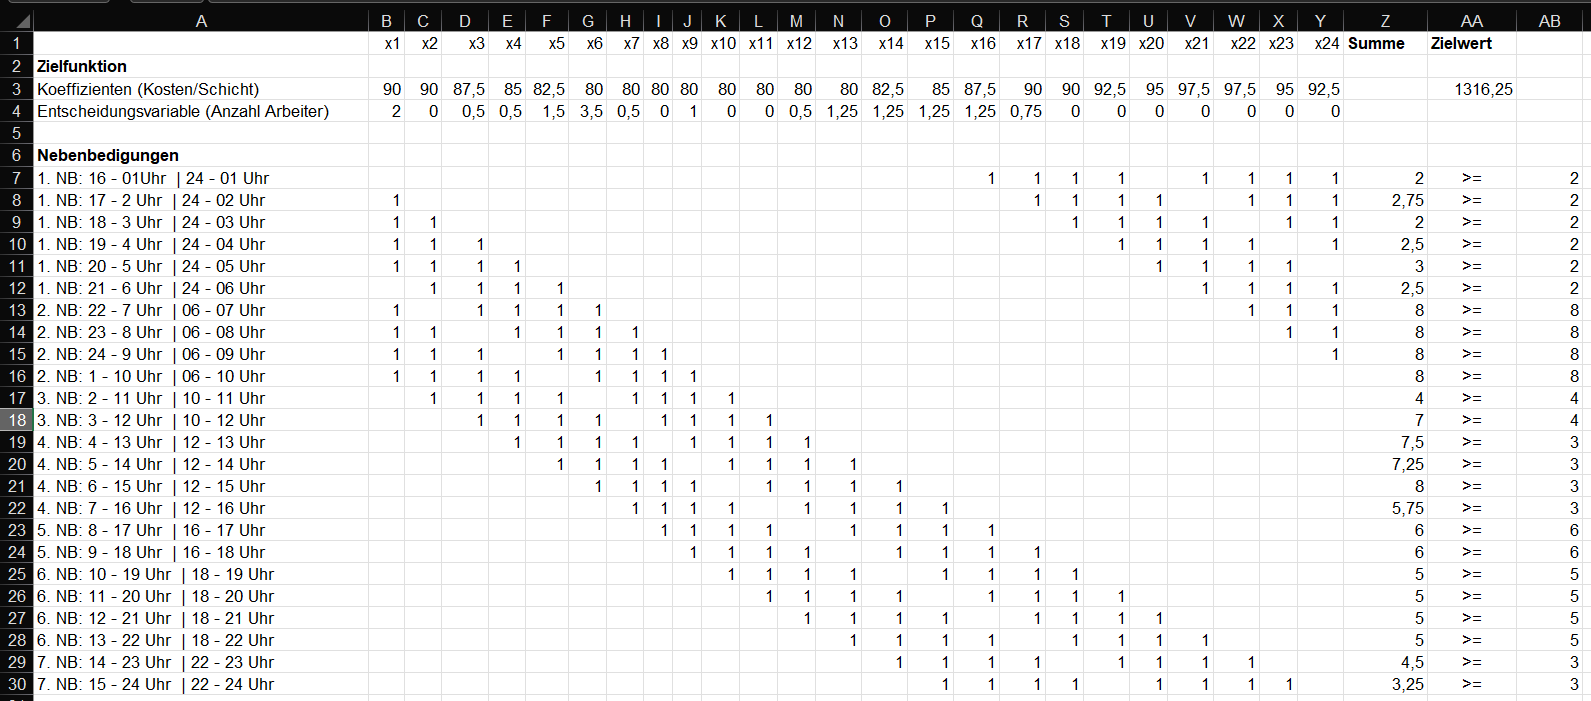
\includegraphics[width=17cm,left]{images/Excel_dezimal.png}\\\\
\\\\
\\\\
\\\\
Ganzzahlige Optimallösung in Excel:\\
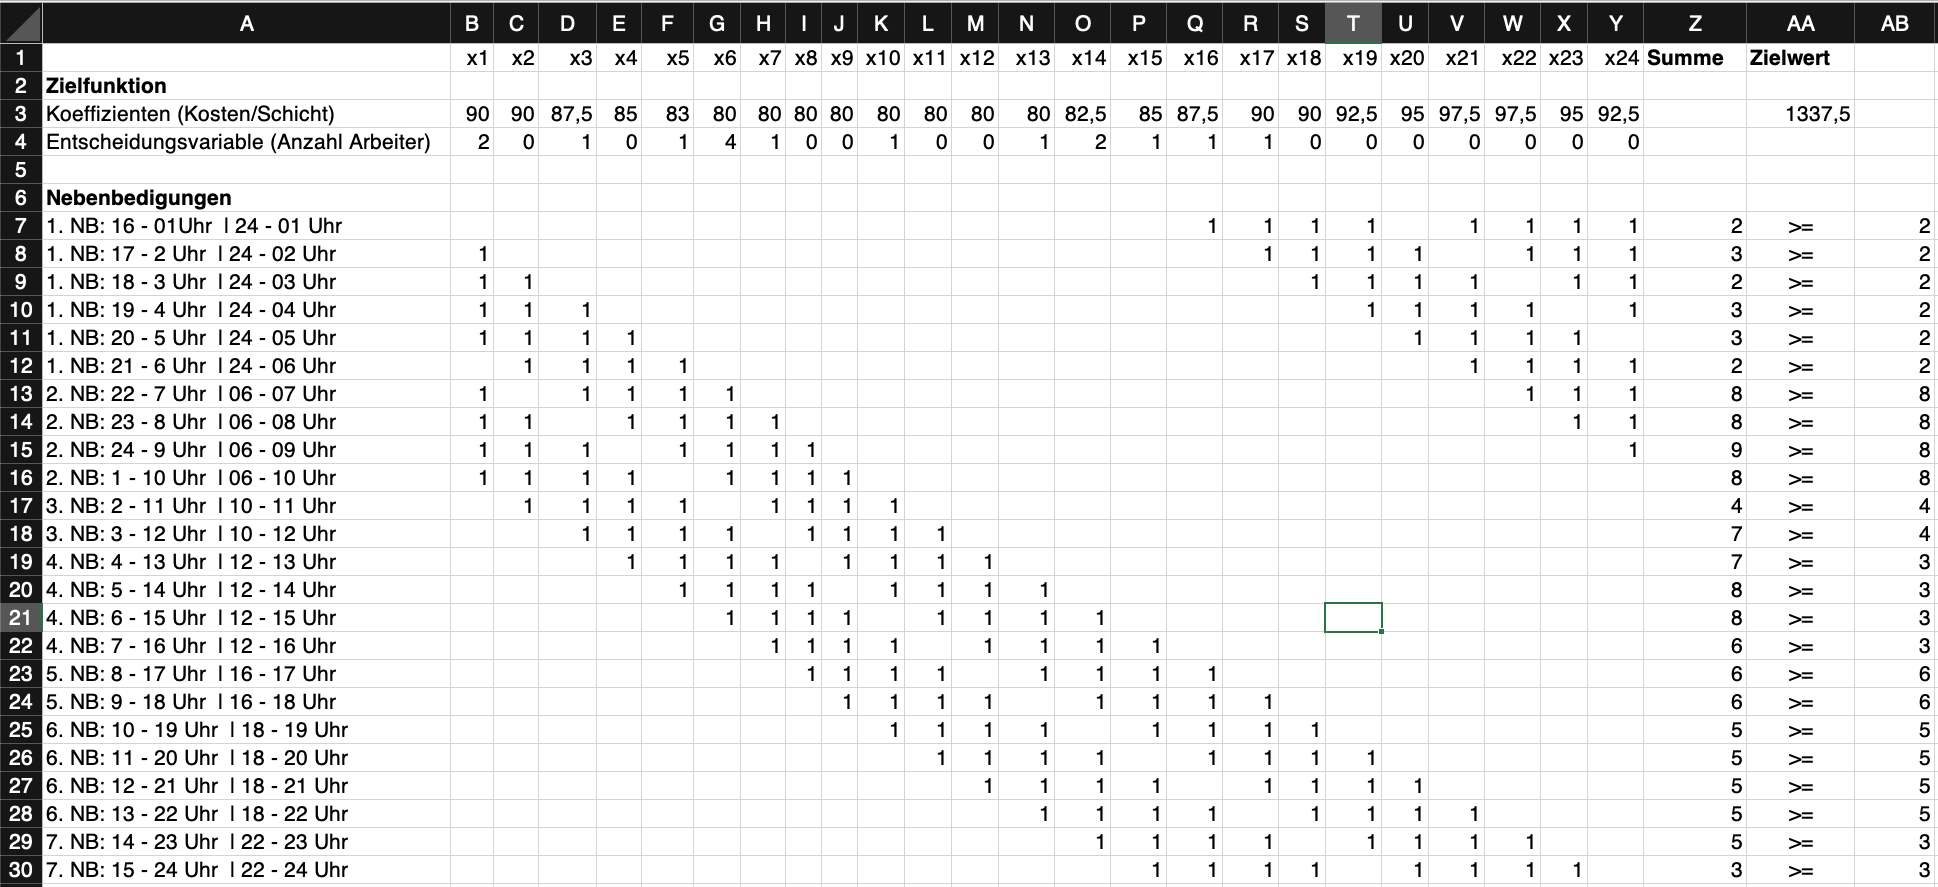
\includegraphics[width=17cm,left]{images/Excel_Ganzzahl.png}\\\\
\pagebreak
\subsection{Sensitivitätsanalyse}
Bei der Sensitivitätsanalyse wird jeweils für die Entscheidungsvariablen sowie den rechten Seiten der Nebenbedingungen, eine zulässige Erhöhung und Verringerung ermittelt. Für die Entscheidungsvariablen: In diesem Intervall dürfen die Werte geändert werden, ohne dass die Optimalitätseigenschaft verloren geht und ein weiterer Iterationsschritt zur Wiederherstellung dieser notwendig ist. Dadurch würden sich in unserem Beispiel die Schichten der Arbeiter anders bezahlen lassen, ohne die Optimalität zu verlieren.\\
Im Fall der Nebenbedingungen: Der Schattenpreis und ein Intervall, in dem der Schattenpreis stabil bleibt, also Aussagen zu den Gesamtlohnkosten getroffen werden können.\\
\\\\
Die Sensitivitätsanalyse unserer Optimalfunktion ergibt folgende Lösung:\\

Für die Entscheidungsvariablen\\

\includegraphics[width=17cm,left]{images/Sensitivitätsbericht_EV.png}\\\\
Hier abzulesen sind bei den Entscheidungsvariablen die Endgültigen Endwerte (Spalte 2), sprich wie viel Personal zu welchem Lohn eingestellt werden muss, sowie die zulässige Erhöhung/Verringerung (Spalte 5 u. 6), in welcher dieser variiert werden kann, ohne die Optimalität zu verlieren. Zu beachten gilt es, dass diese Werte gerundet dargestellt sind und für genaue Angaben in die Zellen geklickt werden muss.\\
Bei Schichtbeginn um 6Uhr (Entscheidungsvariable 6) müssen beispielsweise 3,5 Arbeiter zu einem Lohn von 80€ eingestellt werden. Dieser könnte bis auf ca. 90€ erhöht werden, was nur den Anstieg des Zielfunktionskoeffizienten zur Folge hätte, ohne dass eine neue Verteilung der Entscheidungsvariablen sinnvoller ist. „1E+30“ ist Excels Schreibweise für Unendlich, welche dadurch begründet werden kann, dass zu diesen Zeiten keine Arbeiter eingestellt werden (Wert = 0 in Spalte 2) und somit ein erhöhter Lohn keinen Einfluss auf die Zielfunktion hat.\\
\\\\
Für die Nebenbedingungen\\
\includegraphics[width=17cm,left]{images/Sensitivitätsbericht_NB.png}\\\\
Für die Nebenbedingungen bedeutet der Endgültige Endwert (Spalte 2), die Anzahl an Arbeitern, welche für diese Schicht im Unternehmen eingeteilt sind. Zum Beispiel sind für die Schicht von 1 – 10 Uhr (Spalte 4) 8 Arbeiter eingeteilt, welche zwischen 6 und 10 Arbeitern variiert werden könnten. Auch hier gilt es wieder die gerundete Darstellung zu beachten. Im Gegensatz zu den Entscheidungsvariablen von zuvor, hat hier die Veränderung der Nebenbedingungen auch eine Veränderung der Variablen zur Folge, denn die zulässige Erhöhung/Verringerung gibt uns nur Auskunft darüber, in welchem Intervall der Schattenpreis stabil bleibt.\\
\\
Außerdem wird hier nochmal deutlich, dass die Optimallösung $(x_1=2, x_3=0,5, x_4=0,5, x_5=1,5, x_6=3,5, x_7=0,5, x_9=1, x_{12}=0,5, x_{13}=1,25, x_{14}=1,25, x_{15}=1,25, x_{16}=1,25, x_{17}=0,75; p=1316,25)$ eine dezimale Lösung ist, welche in unserem Sachzusammenhang jedoch nicht sinnvoll ist.\\
\\
Aufgrund dessen wird im Folgenden mit einer nahezu optimalen ganzzahligen Lösung weitergerechnet: $(x_1=2, x_3=1, x_5=1, x_6=4, x_7=1, x_{10}=1, x_{13}=1, x_{14}=2, x_{15}=1, x_{16}=1, x_{17}=1; p=1337,5)$.\\ 
Direkt zu erkennen ist die Veränderung der Entscheidungsvariablen sowie des Zielwertes. Außerdem beträgt die Anzahl der Gesamtbeschäftigten nun 16 Arbeiter statt 15,75, also 0,25 Arbeiter zu viel.\\
\\
Eine Erhöhung der Arbeiter in den 4 Stunden Schichten um einen Arbeiter führt zu einer neuen Lösung mit den Werten: $(x_1=1, x_3=1, x_4=1, x_6=6, x_7=1, x_{10}=1, x_{12}=1, x_{13}=1, x_{14}=2, x_{15}=1, x_{16}=1, x_{18}=1; p=1490,)$ was eine Kostenerhöhung von 153€ zur Folge hätte.\\




